\pagebreak
\section{Question 2}
	
	\subsection{Hough Transform Wall Window}
	\lstinputlisting{./code/Q2/q2a.m}
	\linebreak
	
	
	Using the following image:
	\begin{figure}[position = here]
		\begin{centering}
			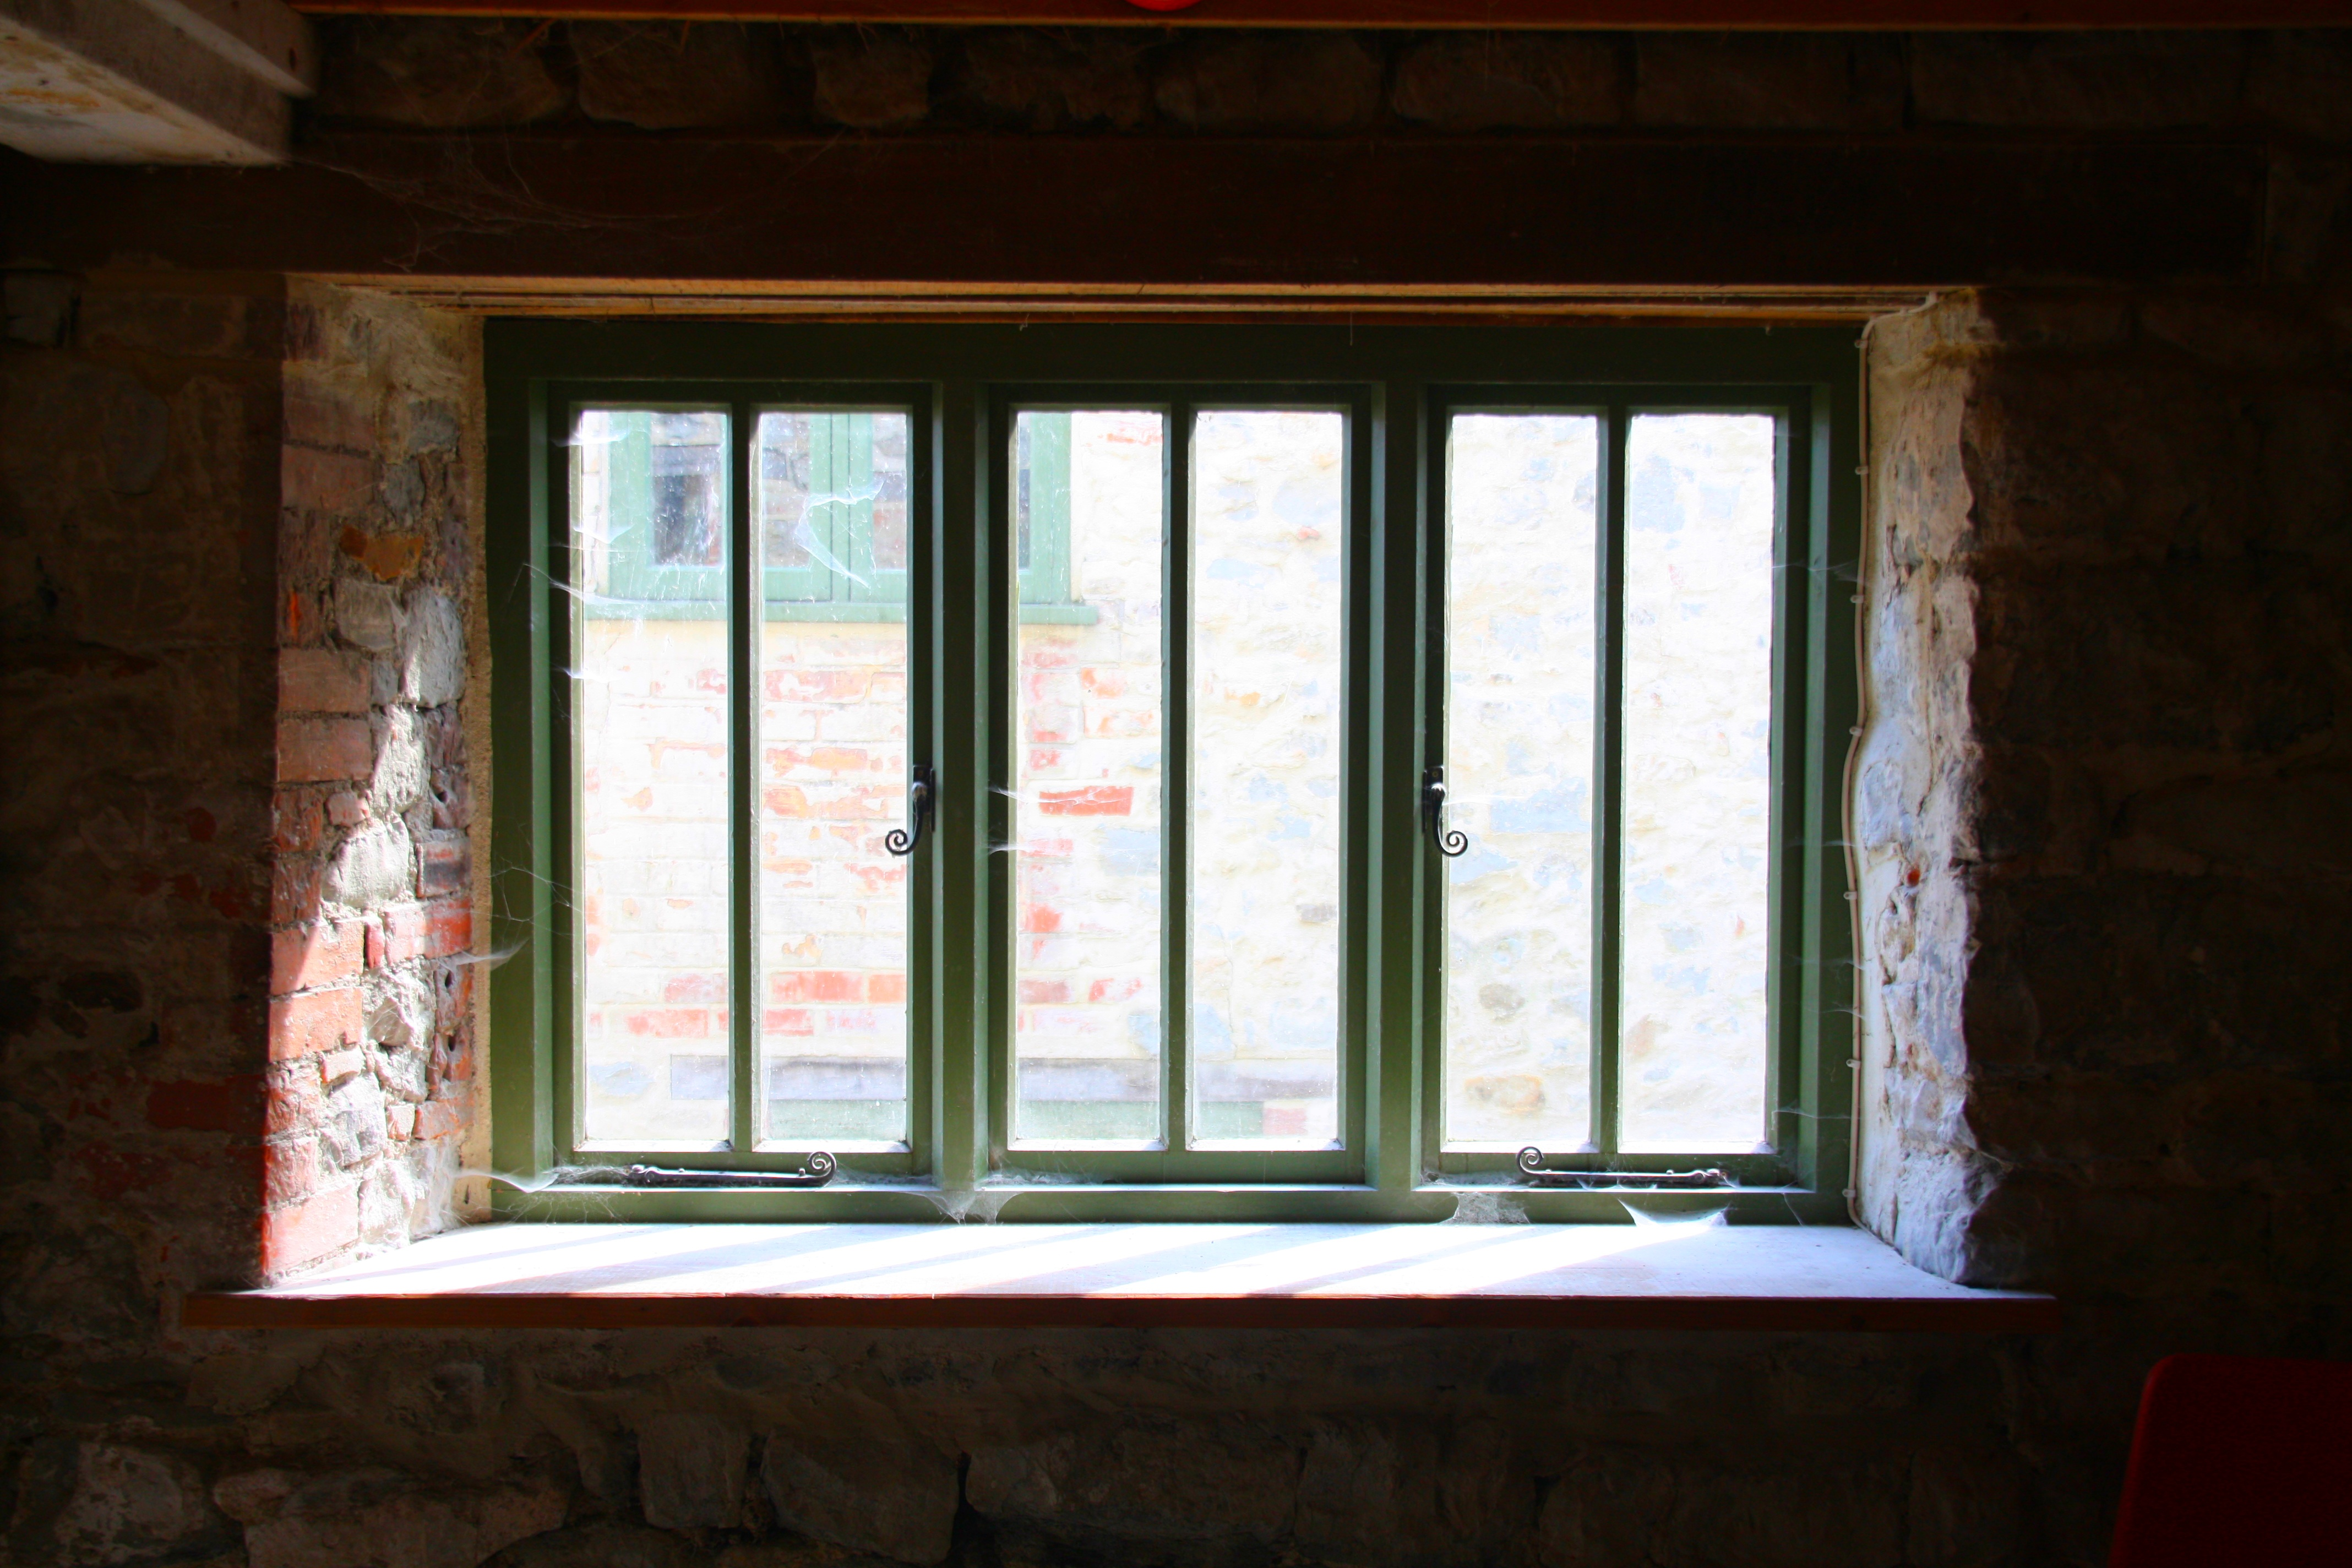
\includegraphics[scale=0.05]{wallWindow}\\
			\caption[\textit{RPYAxes}]{}
		\end{centering}
	\end{figure}
	\newline
		
	\begin{figure}[position = here]
		\begin{centering}
			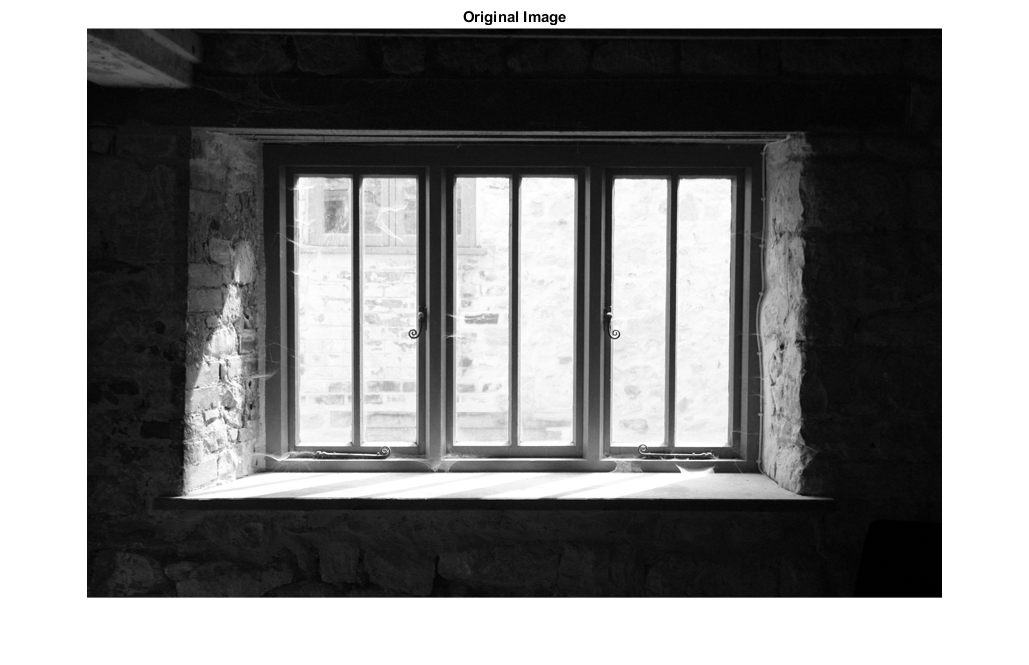
\includegraphics[scale=0.5]{q2a1}\\
			\caption[\textit{RPYAxes}]{}
		\end{centering}
	\end{figure}
	\newline	
	
	\begin{figure}[position = here]
		\begin{centering}
			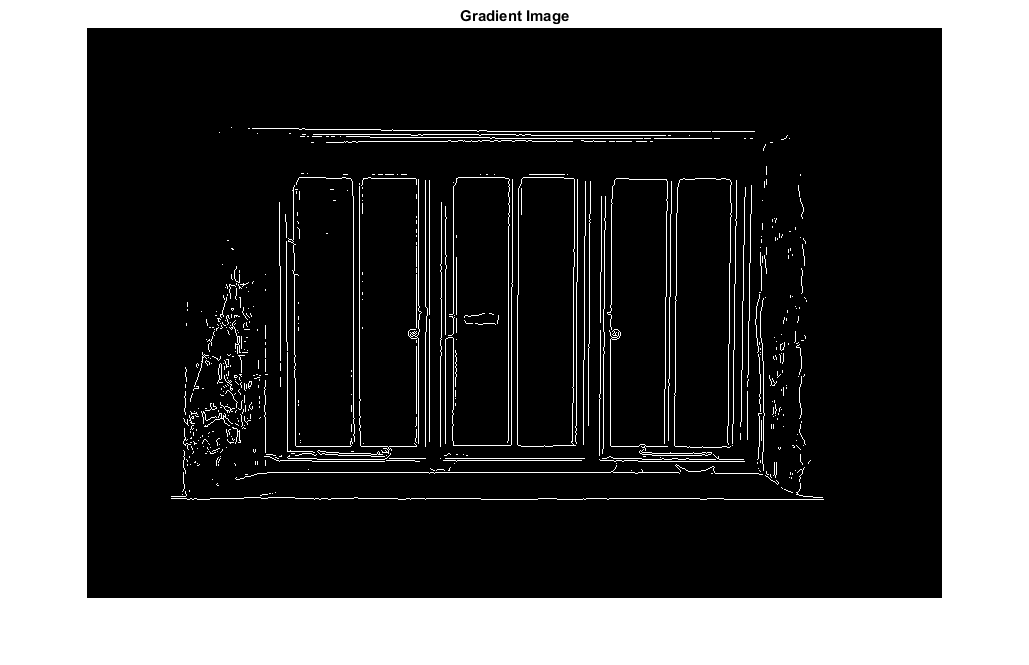
\includegraphics[scale=0.5]{q2a2}\\
			\caption[\textit{RPYAxes}]{}
		\end{centering}
	\end{figure}
	\newline
	
	\begin{figure}[position = here]
		\begin{centering}
			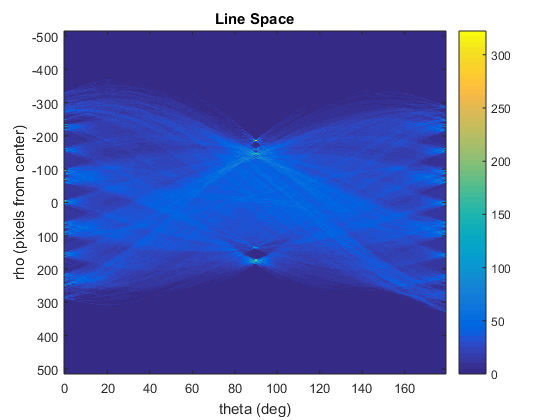
\includegraphics[scale=0.5]{q2a3}\\
			\caption[\textit{RPYAxes}]{}
		\end{centering}
	\end{figure}
	\newline
	
	\begin{figure}[position = here]
		\begin{centering}
			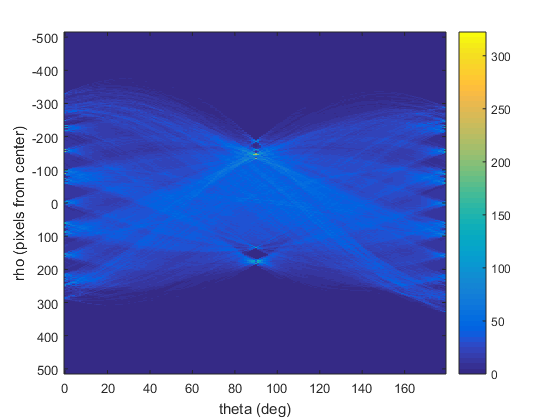
\includegraphics[scale=0.5]{q2a4}\\
			\caption[\textit{RPYAxes}]{}
		\end{centering}
	\end{figure}
	\newline
	
	\begin{figure}[position = here]
		\begin{centering}
			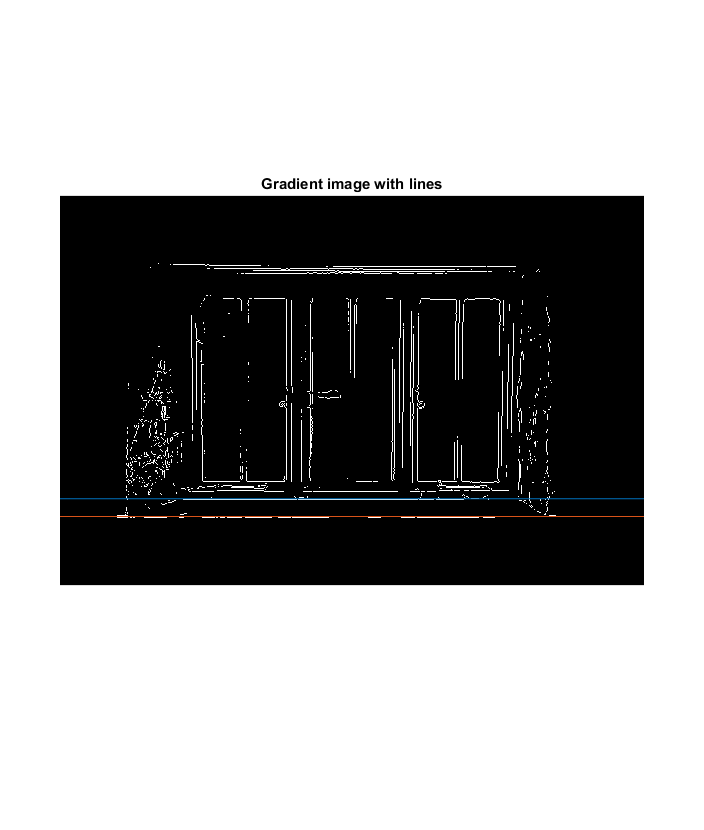
\includegraphics[scale=0.5]{q2a5}\\
			\caption[\textit{RPYAxes}]{}
		\end{centering}
	\end{figure}
	\newline				
	
	\pagebreak
	\subsection{Hough Transform}
	
	\lstinputlisting{./code/Q2/q2b.m}
	\linebreak
	
	\begin{figure}[position = here]
	\begin{centering}
		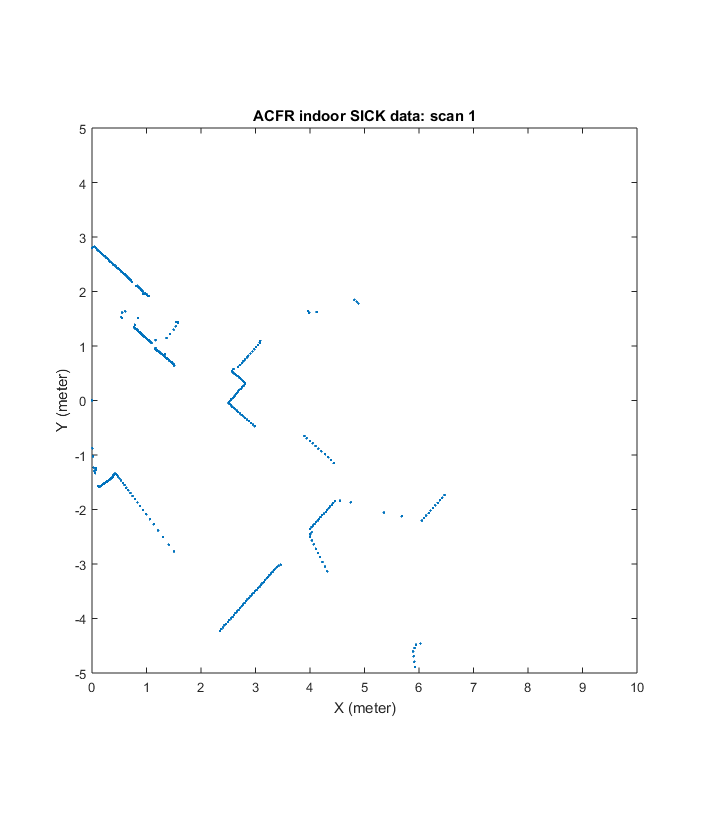
\includegraphics[scale=0.5]{q2b1}\\
		\caption[\textit{RPYAxes}]{}
	\end{centering}
\end{figure}
\newline	

\begin{figure}[position = here]
\begin{centering}
	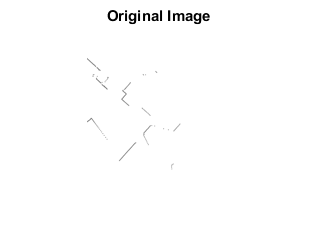
\includegraphics[scale=1]{q2b2}\\
	\caption[\textit{RPYAxes}]{}
\end{centering}
\end{figure}
\newline	

\begin{figure}[position = here]
\begin{centering}
	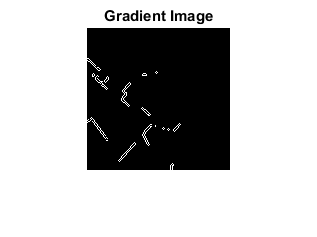
\includegraphics[scale=1]{q2b3}\\
	\caption[\textit{RPYAxes}]{}
\end{centering}
\end{figure}
\newline	


\begin{figure}[position = here]
\begin{centering}
	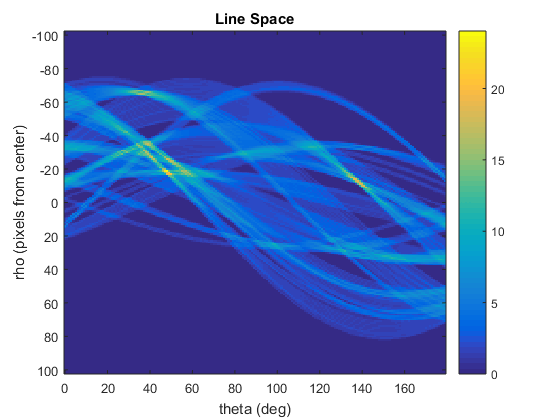
\includegraphics[scale=0.5]{q2b4}\\
	\caption[\textit{RPYAxes}]{}
\end{centering}
\end{figure}
\newline	


\begin{figure}[position = here]
\begin{centering}
	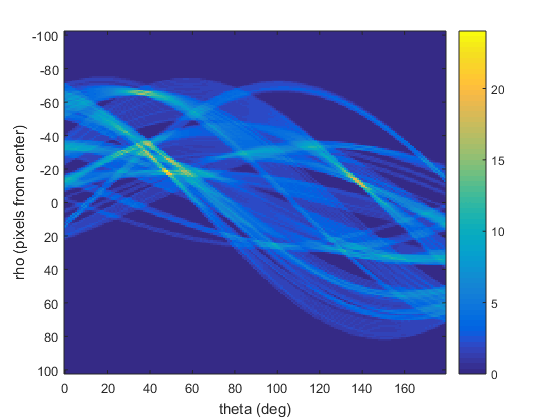
\includegraphics[scale=0.5]{q2b5}\\
	\caption[\textit{RPYAxes}]{}
\end{centering}
\end{figure}
\newline	


\begin{figure}[position = here]
\begin{centering}
	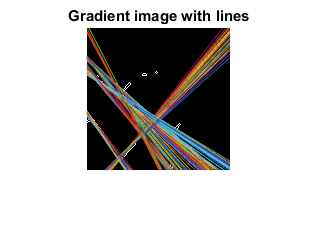
\includegraphics[scale=1]{q2b6}\\
	\caption[\textit{RPYAxes}]{}
\end{centering}
\end{figure}
\newline